\documentclass[12pt,oneside,reqno]{ta-its}
\usepackage{hyperref}
\usepackage{listings}
\usepackage{float}
\usepackage{mdframed}
\usepackage{wrapfig}

\renewcommand{\lstlistingname}{Kode Sumber}
\renewcommand{\lstlistlistingname}{DAFTAR KODE SUMBER}

\title{Rancang Bangun Sistem Monitoring Perangkat Pusat Data Institut Teknologi Sepuluh Nopember (ITS) Surabaya dengan Implementasi Publish-Subscribe dan Telegram API}{Device Monitoring System Design for Data Center of Institut Teknologi Sepuluh Nopember (ITS) Surabaya Using Publish-Subscribe and Telegram API Implementation}{KI141502}

\author{Nafia Rizky Yogayana}{05111440000017}

\supervisorOne{Royyana Muslim Ijtihadie, S.Kom, M.Kom, PhD}{197708242006041001}
\supervisorTwo{Henning Titi Ciptaningtyas, S.Kom, M.Kom.}{198407082010122004}

\degree{Sarjana Komputer}{Arsitektur dan Jaringan Komputer}{S1}{ Informatika}{Informatics}{Teknologi Informasi dan Komunikasi}{FTIK}{Information Technology and Communication}

\time{Juni}{2018}

\begin{document}
\setcounter{tocdepth}{5}
\setcounter{secnumdepth}{5}
\titleformat{\paragraph}[hang]{\normalfont\normalsize\bfseries}{\theparagraph}{1em}{}
\titlespacing*{\paragraph}{0pt}{3.25ex plus 1ex minus .2ex}{0.5em}
\renewcommand{\thelstlisting}{\arabic{chapter}.\arabic{lstlisting}}
	\frontmatter % Halaman dengan penomoran romawi kecil
	\maketitle
	\legalityPaper % Lembar Pengesahan
	
    \begin{abstrak}
Seiring dengan perkembangan zaman yang sangat pesat, negara-negara sudah mempunyai teknologi yang sangat maju. Teknologi mempunyai peranan yang sangat penting dalam kehidupan manusia, karena dengan adanya teknologi, manusia bisa saling berhubungan dengan mudah. Sekarang teknologi sudah semakin canggih. Teknologi yang paling populer sekarang ini adalah internet karena dengan adanya internet, banyak informasi-informasi yang dapat kita ambil dengan mudah. Internet merupakan suatu perpustakaan besar yang di dalamnya terdapat sangat banyak informasi yang berupa teks dalam bentuk media elektronik. Selain itu internet dikenal sebagai dunia maya, karena hampir seluruh aspek kehidupan di dunia nyata ada di internet, seperti olah raga, politik, hiburan, akademik, bisnis, dan lain sebagainya. Internet juga mempunyai peranan yang sangat penting dalam dunia pendidikan, karena dengan adanya internet bisa menambah ilmu pengetahuan kita dan dapat menambah motivasi belajar siswa ataupun mahasiswa. Dengan dimanfaatkan itnernet dalam dunia pendidikan agar siswa atau mahasiswa dapat memiliki komitmen untuk belajar secara aktif dan memiliki teknis kemampuan khususnya di bidang pendidikan. Oleh karena itu, internet dapat mempermudah proses belajar mengajar dengan baik.

Dalam dunia pendidikan, internet telah menjadi platform penting, misalnya adalah proses belajar mengajar yang dilakukan secara online dengan e-learning, ataupun ketika pengajar memberikan nilai kepada siswanya dilakukan secara online, dan lain sebagainya. Keamanan menjaga data-data dalam dunia pendidikan, melindungi terhadap penggunaan malware, menerapkan kepatuhan akses internet, menyederhanakan manajemen jaringan menjadi tantangan utama untuk manajemen TI. Maka dari itu dibutuhkan sebuah server yang digunakan sebagai internet access management atau untuk melakukan manajemen akses terhadap user yang menggunakan jaringannya.

Namun akan terjadi permasalahan ketika banyak user yang mengakses internet dengan menggunakan server yang digunakan sebagai internet access management. Dalam pembacaan log history dari setiap user akan tercampur karena hanya melewati satu server saja. 

Dalam tugas akhir ini akan dibuat sebuah rancangan sistem pada server yang akan dijadikan sebagai internet access management, yang memungkinkan untuk mencatat setiap log history dari setiap user yang mengakses internet secara detail. Rancangan sistem pada server akan menggunakan kontainer docker. Kontainer docker merupakan operating-system-level virtualization untuk menjalankan beberapa sistem linux yang terisolasi (kontainer) pada sebuah host. Kontainer berfungsi untuk mengisolasi aplikasi atau servis dan dependensinya. Untuk setiap servis atau aplikasi yang terisolasi dibutuhkan satu kontainer pada server host yang ada dan setiap kontainer akan menggunakan sumber daya yang ada pada server host selama kontainer tersebut menyala.\\

	\noindent \textbf{Kata-Kunci}: Docker, Internet Access Management, Kontainer
\end{abstrak}
\newpage
\begin{abstract}
Along with the rapid development of the era, the countries already have advanced technology. Technology has a very important role in human life, because with technology, humans can interconnect easily. Now, technology is getting more sophisticated. The most popular technology today is internet, because with  internet, we can take a lot of information easily. Internet is one of the very many media information that contains text in the form of electronic media. In addition, internet is known as virtual word, because various aspects of life in the world, such as sports, politics, entertainment, educations, business, etc. Internet also has a very important role in the world of education, because internet can increase our knowledge and can increase students motivation to learn. Therefor, internet can help learning process well.

Internet has become a vital platform for most educations, for example is the process of teaching and learning that is done oneline with e-learning, or when teachers / lecturers provide score to their students are done online, etc. Safe guarding data, protecting against malware usages, implementing internet access compliance, simplifying network management become the key challenges for IT management. Therefore required a server that is used as internet access management or to perform management access to users who use the network.

But there will be problems when many users who access internet by using a server that is used as internet access management. In reading log history of each user will be mixed because only through one server only.

In this final project will be created a system design on the server that will serve as internet access management, which allows to record every log history of each user who access internet in detail. The system design on the server will user docker containers. Docker containers is an operating system level virtualization to run some isolated linux systems (containers) on a host. Containers are used to isolate applications or services and its dependencies. For every service or app that isolated it takes one container on the existing host server and each container will user the existing resources on the host server as long as the container is on.\\

	\noindent \textbf{Keywords}: Container, Docker, Internet Access Management
\end{abstract}
	\chapter{Kata Pengantar}
		\begin{figure}[h]
			\centering
			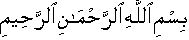
\includegraphics[width=0.5\linewidth]{img/bismillah.png}
		\end{figure}

		Alhamdulillahirabbil’alamin, segala puji bagi Allah SWT, yang telah melimpahkan rahmat dan hidayah-Nya sehingga penulis dapat menyelesaikan Tugas Akhir yang berjudul \textbf{Rancang Bangun Perangkat Lunak Internet \textit{Acces Management} Berbasis Kontainer}. Pengerjaan Tugas Akhir ini merupakan suatu kesempatan yang sangat baik bagi penulis. Dengan pengerjaan Tugas Akhir ini, penulis bisa belajar lebih banyak untuk memperdalam dan meningkatkan apa yang telah didapatkan penulis selama menempuh perkuliahan di Teknik Informatika ITS. Dengan Tugas Akhir ini penulis juga dapat menghasilkan suatu implementasi dari apa yang telah penulis pelajari.
		Selesainya Tugas Akhir ini tidak lepas dari bantuan dan dukungan beberapa pihak. Sehingga pada kesempatan ini penulis mengucapkan syukur dan terima kasih kepada:
		\begin{enumerate}
			\item Allah SWT atas anugerahnya yang tidak terkira kepada penulis dan Nabi Muhammad SAW.
			\item Bapak, Mama, dan keluarga Penulis yang selalu memberikan perhatian, dorongan dan kasih sayang yang menjadi semangat utama bagi diri Penulis sendiri baik selama penulis menempuh masa perkuliahan maupun pengerjaan Tugas Akhir ini.
			\item Bapak Royyana Muslim Ijtihadie, S.Kom., M.Kom., PhD. selaku Dosen Pembimbing yang telah banyak meluangkan waktu untuk memberikan ilmu, nasihat, motivasi, pandangan dan bimbingan kepada Penulis baik selama Penulis menempuh masa kuliah maupun selama pengerjaan Tugas Akhir ini.
			\item Bagus Jati Santoso, S.Kom., PhD. selaku dosen pembimbing yang telah memberikan ilmu, dan masukan kepada Penulis.
			\item Seluruh tenaga pengajar dan karyawan Jurusan Teknik Informatika ITS yang telah memberikan ilmu dan waktunya demi berlangsungnya kegiatan belajar mengajar di Jurusan Teknik Informatika ITS.
			\item Seluruh teman Penulis di Jurusan Teknik Informatika ITS yang telah memberikan dukungan dan semangat kepada Penulis selama Penulis menyelesaikan Tugas Akhir ini.
			\item Teman-teman, Kakak-kakak dan Adik-adik \textit{administrator} Laboratorium Arsitektur dan Jaringan Komputer yang selalu menjadi teman untuk berbagi ilmu.
		\end{enumerate}

		Penulis menyadari bahwa Tugas Akhir ini masih memiliki banyak kekurangan. Sehingga dengan kerendahan hati, penulis mengharapkan kritik dan saran dari pembaca untuk perbaikan ke depannya.

		\hfill Surabaya, Juni 2018 \\ \\
		\hfill Fourir Akbar

	\cleardoublepage % Mengisi penanda halaman genap yang kosong

	\tableofcontents % Daftar Isi
	\listoftables % Daftar Tabel
	\listoffigures % Daftar Gambar
	\lstlistoflistings % Daftar Kode Sumber

	\mainmatter
	\chapter{PENDAHULUAN}
Pada bab ini akan dijelaskan latar belakang, rumusan masalah, batasan masalah, tujuan, manfaat, metodologi dan sistematika penulisan Tugas Akhir.

\section{Latar Belakang}
\textit{Monitoring} adalah suatu kegiatan yang meliputi observasi dan pengecekan terhadap kemajuan suatu proses atau kualitas dari suatu barang atau pekerjaan dan dilakukan secara berkala. Banyak hal yang bisa dimonitor, mulai dari barang, kesehatan, hingga pekerjaan. Untuk keperluan Tugas Akhir ini, \textit{monitoring} dilakukan terhadap perangkat yang ada di Pusat Data Institut Teknologi Sepuluh Nopember (ITS) Surabaya, yakni server dan komputer \textit{single-board}. Tujuan dari adanya \textit{monitoring} ini adalah untuk memantau jaringan dan lingkungan di Pusat Data ITS.

\textit{Monitoring} server adalah kegiatan memantau sebuah server dari segi kinerja perangkat keras, \textit{traffic} lalu lintas data, dan masih banyak lagi. \textit{Monitoring} server ini merupakan suatu pekerjaan yang sangat penting untuk dilakukan dalam memanajemen jaringan. \textit{Monitoring} ini menjadi suatu titik yang menentukan apakah suatu layanan jaringan sudah berjalan dengan baik atau tidak.

Dalam suatu kegiatan \textit{monitoring} server, tidak semua pengguna layanan bisa melakukan hal tersebut karena terkait dengan hak akses masing-masing. Dan dalam pelaksanaannya selama ini, \textit{monitoring} server dilakukan secara manual dan tidak seragam. Hal ini yang menyebabkan administrator merasa kesulitan dalam mengatasi masalah jaringan yang terjadi.

Selain itu, lingkungan di Pusat Data ITS juga perlu dipantau. Amat sulit rasanya jika administrator harus memantau dari komputer \textit{single-board} secara manual. Pekerjaan ini membutuhkan ekstra waktu. Dan belum tentu juga administrator langsung mengetahui jika ada server yang \textit{down} atau keadaan lain yang membutuhkan penanganan langsung.

Berdasarkan uraian di atas maka dapat dilihat bahwa dibutuhkan sebuah sistem untuk menangani masalah \textit{monitoring} perangkat yang ada di Pusat Data ITS ini. Dengan adanya sistem yang seragam, diharapkan dapat membantu para administrator dalam memantau server dan komputer \textit{single-board} dengan lebih mudah dan efisien.


\section{Rumusan Masalah}
Rumusan masalah yang diangkat dalam Tugas Akhir ini adalah sebagai berikut:
\begin{enumerate}
	\item Bagaimana cara membangun sistem administrasi \textit{monitoring} untuk pemantauan server?
	\item Bagaimana cara mengimplementasikan \textit{publish-subscribe} pada monitoring server?
	\item Bagaimana cara membangun \textit{agent} yang melaporkan keadaan server ke pengguna?
	\item Bagaimana cara mengambil informasi penggunaan CPU, memori, \textit{bandwidth}, dan hal-hal lain yang terkait pada server?
	\item Bagaimana cara mengimplementasikan \textit{publish-subscribe} pada komputer papan tunggal (\textit{single board computer}) untuk pemantauan lingkungan Pusat Data ITS?
	\item Bagaimana cara mengintegrasikan antara \textit{agent} ke Telegram untuk mengirim notifikasi mengenai keadaan lingkungan atau server di Pusat Data ITS yang membutuhkan penanganan langsung?
\end{enumerate}

\section{Batasan Masalah}
Permasalahan yang dibahas pada Tugas Akhir ini memiliki beberapa batasan, yaitu sebagai berikut:

\begin{enumerate}
	\item Sistem hanya melakukan \textit{monitoring} pada Linux Server dan Raspberry Pi sebagai komputer \textit{single-board} untuk membaca sensor.
	\item Sistem ini diimplementasikan di Pusat Data Institut Teknologi Sepuluh Nopember (ITS) Surabaya.
\end{enumerate}

\section{Tujuan}
Tujuan dari Tugas Akhir ini adalah sebagai berikut:

\begin{enumerate}
	\item Membuat sebuah sistem \textit{monitoring} untuk perangkat di Pusat Data ITS berupa server dan komputer \textit{single-board} yang seragam untuk seluruh pengguna.
	\item Mengimplementasikan metode \textit{publish-subscribe} pada sistem \textit{monitoring} server dan komputer \textit{single-board} di Pusat Data ITS.
\end{enumerate}

\section{Manfaat}
Manfaat dari Tugas Akhir ini adalah sebagai berikut:

\begin{enumerate}
	\item Membangun sebuah sistem administrator \textit{monitoring} server dan komputer \textit{single-board} agar memudahkan para admin dalam memantau server yang ada.
	\item Membangun sistem administrator untuk memantau lingkungan Pusat Data ITS dengan sensor yang dihubungkan ke Raspberry Pi.
	\item Memonitoring server dan yang hanya ingin dimonitoring dengan cara memilih saluran server yang ada.
	\item Membangun \textit{agent} dengan sistem \textit{publish-subscribe} agar dapat melaporkan keadaan server ke pengguna.
	\item Membangun \textit{agent} untuk diletakkan di komputer \textit{single-board} agar bisa melaporkan keadaan lingkungan Pusat Data ITS ke pengguna dengan mengimplementasikan \textit{publish-subscribe}.
	\item Mengetahui informasi seperti penggunaan CPU, memori, \textit{bandwidth}, dan hal lain yang terkait pada server dengan adanya sistem \textit{monitoring} server ini.
	\item Memberitahu pengguna tentang keadaan server atau lingkungan Pusat Data ITS yang butuh perhatian langsung melalui aplikasi Telegram.
\end{enumerate}

\section{Metodologi}
Metodologi yang digunakan pada pengerjaan Tugas Akhir ini
adalah sebagai berikut:
\subsection{Penyusunan Proposal Tugas Akhir}
Tahap awal untuk memulai pengerjaan Tugas Akhir adalah penyusunan proposal Tugas Akhir yang berisi gagasan untuk menyelesaikan permasalahan di Pusat Data ITS Surabaya.

Proposal tugas akhir ini berisi tentang deskripsi pendahuluan dari tugas akhir yang akan dibuat. Pendahuluan ini terdiri atas hal yang menjadi latar belakang diajukannya usulan tugas akhir, rumusan masalah yang diangkat, batasan masalah untuk tugas akhir, tujuan dari pembuatan tugas akhir, dan manfaat dari hasil pembuatan tugas akhir. Selain itu dijabarkan pula tinjauan pustaka yang digunakan sebagai referensi pendukung pembuatan tugas akhir. Sub bab metodologi berisi penjelasan mengenai tahapan penyusunan tugas akhir mulai dari penyusunan proposal hingga penyusunan buku tugas akhir. Terdapat pula sub bab jadwal kegiatan yang menjelaskan jadwal pengerjaan tugas akhir.
\subsection{Studi literatur}
Studi literatur merupakan langkah yang dilakukan untuk mendukung dan memastikan setiap tahap pengerjaan tugas akhir sesuai dengan standar dan konsep yang berlaku. Pada tahap studi literatur ini, akan dilakukan studi mendalam mengenai \textit{monitoring} server, Raspberry Pi, dan \textit{Publish-Subscribe}. Adapun literatur yang dijadikan sumber berasal dari paper, buku, materi perkuliahan, forum serta artikel dari internet.
\subsection{Desain dan Perancangan Sistem}
Pada tahap ini dilakukan desain dan perancangan sistem \textit{monitoring} perangkat di Pusat Data ITS Surabaya.

Aktor dari aplikasi ini adalah administrator yang akan melakukan \textit{monitoring} server dan komputer \textit{single-board}. Admin memilih server atau perangkat mana yang ingin ia pantau. Dari permintaan tersebut, maka sistem akan memberikan informasi perangkat terpilih kepada pengguna yang memilih perangkat tersebut.

Tahap ini merupakan tahap yang paling penting dimana bentuk awal aplikasi yang akan diimplementasikan didefinisikan. Pada tahapan ini dibuat desain dari arsitektur sistem.
\subsection{Implementasi Sistem}
Implementasi merupakan tahap membangun dan  mengimplementasikan rancangan sistem yang telah dibuat. Pada tahapan ini merealisasikan apa yang telah didesain dan dirancang pada tahapan sebelumnya, sehingga menjadi sebuah sistem yang sesuai dengan apa yang telah direncanakan.
\subsection{Uji Coba dan Evaluasi}
Pada tahapan ini dilakukan uji coba terhadap sistem yang telah dibuat. Pengujian dan evaluasi akan dilakukan dengan melihat kesesuaian dengan perencanaan. Selain itu, tahap ini juga akan melakukan uji performa sistem untuk mengetahui efisiensi penggunaan sumber daya serta evaluasi berdasarkan hasil uji performa tersebut.

Pengujian dalam aplikasi ini akan dilakakukan dalam beberapa cara, antara lain:
\begin{itemize}
	\item Pengujian pada keberhasilan dalam mengambil informasi dari tiap-tiap server (\textit{monitoring} server).
	\item Pengujian pada keberhasilan dalam pengambilan informasi dari komputer \textit{single-board} untuk memantau lingkungan Pusat Data ITS.
	\item Pengujian ini berfokus pada ketepatan informasi dari hasil \textit{monitoring} perangkat dan diberikan (\textit{publish}) ke pengguna yang meminta (\textit{subscribe}).
\end{itemize}
\subsection{Penyusunan Buku Tugas Akhir} 
Pada tahap ini dilakukan penyusunan buku Tugas Akhir yang berisi dokumentasi hasil pengerjaan Tugas Akhir.


\section{Sistematika Penulisan}
Berikut adalah sistematika penulisan buku Tugas Akhir ini:
\begin{enumerate}
	\item BABI: PENDAHULUAN
	
	Bab ini berisi latar belakang, rumusan masalah, batasan masalah, tujuan, manfaat, metodologi dan sistematika penulisan Tugas Akhir.
	
	\item BAB II: DASAR TEORI
	
	Bab ini berisi dasar teori mengenai permasalahan dan algoritma penyelesaian yang digunakan dalam Tugas Akhir
	
	\item BAB III: DESAIN
	
	Bab ini berisi desain algoritma dan struktur data yang digunakan dalam penyelesaian permasalahan.
	
	\item BAB IV: IMPLEMENTASI
	
	Bab ini berisi implementasi berdasarkan desain algortima yang telah dilakukan pada tahap desain.
	
	\item BAB V: UJI COBA DAN EVALUASI
	
	Bab ini berisi uji coba dan evaluasi dari hasil implementasi yang telah dilakukan pada tahap implementasi.
	
	\item BAB VI: PENUTUP
	
	Bab ini berisi kesimpulan dan saran yang didapat dari hasil uji coba yang telah dilakukan.
\end{enumerate}

\cleardoublepage

	\chapter{DASAR TEORI}
Pada bab ini akan dijelaskan mengenai dasar teori yang menjadi dasar pengerjaan Tugas Akhir ini.


\section{Deskripsi Umum}
Pada subbab ini akan dijelaskan mengenai deskripsi-deskripsi umum yang terdapat pada Tugas Akhir ini.

\subsection{SNMP}
SNMP (\textit{Simple Network Management Protocol}) adalah metode “tanpa agen” untuk memonitor perangkat dan server jaringan. Ribuan perangkat jaringan dan sistem operasi yang berbeda dari vendor yang berbeda mendukung SNMP untuk menyampaikan informasi penting yang berhubungan dengan penggunaan, status layanan, dan lainnya.\\
SNMP merupakan pembaharuan dari versi sebelumnya, yakni SGMP (\textit{Simple Gateway Management Protocol}). Protokol ini direncanakan melakukan pertukaran dengan arsitektur \textit{Common Management Information Service/Protocol} (CMIS / CMIP) berdasarkan solusi.

SNMP terdiri dari model manajer/agen yang di dalamnya terdapat manajer SNMP, agen MP dan database informasi manajemen, perangkat SNMP yang dikelola dan protokol jaringan. Manajer SNMP menyediakan antarmuka antara manajer jaringan manusia dan sistem manajemen. Agen SNMP menyediakan antarmuka antara manajer dan perangkat fisik yang sedang dikelola.


\subsection{\textit{Publish-Subscribe}}
Secara umum, maksud dari \textit{publish-subscribe} adalah susunan dari sekumpulan node yang didistribusikan melalui jaringan komunikasi. Klien dari sistem ini dibagi menjadi dua peran yaitu \textit{publisher} dan \textit{subscriber}.

\textit{Publisher} adalah yang penyedia informasi dan memberikannya kepada yang meminta informasi tersebut. Sedangkan \textit{subscriber} bertindak sebagai konsumen informasi tersebut. Dua klien ini tidak diharuskan untuk berkomunikasi secara langsung di antara mereka sendiri yang namun agak terpisah: interaksi terjadi melalui nodes sistem \textit{publish-subscribe}, yang mengkoordinasikan diri mereka untuk mengarahkan informasi dari penerbit ke pelanggan. Pengunaan \textit{publisher} dan \textit{subscriber} ini dapat memungkinkan skalabilitas yang lebih besar dan topologi jaringan yang lebih dinamis.

Terdapat dua jenis \textit{publish-subscribe}, yaitu \textit{topic based} \textit{publish-subscribe} dan \textit{content based} \textit{publish-subscribe}. \textit{Topic based} \textit{publish-subscribe} merupakan pola pengiriman pesan \textit{publish-subscribe} dimana penyedia informasi menyampaikan pesan ke konsumen berdasarkan topik yang dipilihnya. \textit{Content based} \textit{publish-subscribe} merupakan pola pengiriman pesan \textit{publish-subscribe} dimana penyedia informasi menyampaikan pesan ke konsumen berdasarkan isi dari pesan yang ada. Pada umumnya pola pengiriman pesan \textit{publish-subscribe} merupakan \textit{topic based}.


\subsection{\textit{Websocket}}
\textit{Websocket} merupakan protokol komunikasi yang memungkinkan komunikasi dua arah antara \textit{web client} dengan \textit{server}. Penerapan komunikasi dua arah ini dapat digambarkan oleh pengguna telepon. Kedua orang yang sedang bertelepon dapat berbicara dan mendengarkan secara bersamaan dan \textit{real-time}. Protokol \textit{websocket} memungkinkan komunikasi dua arah antara klien dengan \textit{server} secara \textit{real-time}.

Pada umumnya \textit{web client} mendapatkan satu kali tanggapan dari \textit{server} untuk setiap satu permintaan. Alur tersebut kurang tepat apabila digunakan untuk menerapkan pola pengiriman pesan \textit{publish-subscribe} dimana \textit{subscriber} biasanya akan menunggu terus menerus terhadap pesan yang dikirimkan oleh \textit{publisher}. Sedangkan \textit{publisher} mungkin saja mengirimkan pesan lagi setelah 5 menit. Maka dari itu \textit{websocket} digunakan untuk menampilkan secara \textit{real-time} pesan yang diperoleh dari \textit{publisher} walaupun harus menunggu dalam jangka waktu yang tidak pasti.

Untuk membuat koneksi \textit{websocket}, klien harus mengirimkan \textit{request} HTTP kepada \textit{server}. Setelah itu protokol akan diubah menjadi protokol \textit{Websocket}, lalu \textit{server} akan mengenali tipe \textit{request} berdasarkan \textit{header} pada HTTP. Protokol akan diupgrade menjadi \textit{Websocket} apabila diminta. Kemudian klien dan server akan memulai komunikasi \textit{full-duplex}, yang berarti klien dan server dapat bertukar data kapanpun sampai salah satu dari klien atau server menutup koneksi tersebut.


\subsection{Rabbitmq}
Rabbitmq merupakan perantara (broker) pada pertukaran pesan. Rabbitmq juga biasa disebut \textit{message-oriented middleware}. Rabbitmq mendukung pola pengiriman pesan \textit{publish-subscribe}.

Pada arsitektur pola pengiriman pesan \textit{publish-subscribe} yang terdapat di rabbitmq akan sering ditemui istilah-istilah seperti \textit{exchange} dan \textit{queue}. \textit{Exchange} dapat diartikan sebagai persimpangan, sedangkan \textit{queue} dapat diartikan sebagai tempat penyimpanan. Rabbitmq menggunakan istilah \textit{producer} untuk pihak yang membuat pesan untuk nantinya dikirim ke broker dan \textit{consumer} untuk pihak yang nantinya akan menerima pesan dari broker yang dibuat oleh \textit{producer}. \textit{Producer} pada pola pengiriman pesan \textit{publish-subscribe} dikenal dengan istilah \textit{publisher} sedangkan \textit{consumer} dikenal dengan istilah \textit{subscriber}.

Pada arsitektur pola pengiriman pesan \textit{publish-subscribe} pesan yang dibuat oleh \textit{text}publisher mungkin saja dikonsumsi oleh beberapa \textit{subscriber}. \textit{Publisher} nantinya akan mengirim pesan ke suatu \textit{exchange} yang berada pada broker, akan tetapi \textit{exchange} tidak dapat menyimpan pesan. Ketika suatu \textit{exchange} yang dikirimi pesan tidak memiliki \textit{queue} yang tersambung, maka pesan tersebut akan hilang. Pada kasus ini masing-masing \textit{subscriber} akan membuat \textit{queue} yang berbeda untuk menyimpan pesan yang dibuat oleh \textit{publisher}. Oleh rabbitmq pesan yang sudah pernah dipakai (\textit{consume}) akan langsung dihapus dari \textit{queue}.

\subsection{Nagios}
Nagios adalah perangkat lunak open source yang menyediakan alat pemantauan yang sempurna yang dapat membantu untuk memantau seluruh protokol yang aktif dan perangkat jaringan yang terhubung dengan topologi. Nagios juga merupakan sistem pemantauan yang paling yang paling populer yang cocok dengan hampir semua distribusi linux. Aplikasi ini memiliki banyak \textit{plugin} tambahan yang dikembangkan oleh pengguna maupun yang terdapat langsung pada awal pengaturan. Peralatan pemantauan yang berbasis Nagios juga tersedia, seperti sensor yang dirancang untuk beroperasi bersama Nagios. Karena fleksibilitas dari rancangan perangkat lunak yang menggunakan arsitektur \textit{plugin}, layanan pengecekan untuk aplikasi yang pustakanya sudah ditentukan dapat digunakan. Di dalam Nagios terdapat beberapa \textit{plugin} lain, seperti script tambahan yang dapat dikostumisasi dan dapat digunakan pada Nagios. Nagios juga mampu untuk menyediakan grafik yang komperhensif dan bersifat \textit{real-time} dan analisis tren.


\subsection{Raspberry Pi}
Raspberry Pi adalah salah satu jenis \textit{Single-Board Computer} (SBC) yang bisa digunakan dalam sistem pemantauan. Raspberry Pi merupakan SBC yang memiliki \textit{low-power} dengan ukuran sebesar kartu kredit yang dirilis pada tahun 2012. Alat ini bisa dibilang merupakan alat yang paling populer yang dikembangkan oleh Universitas Cambridge UK untuk kepentingan pendidikan komputasi.

Raspberry Pi ini memiliki RAM sebesar $1$ GB, 900 Mhz \textit{quad-core} ARM Cortex A7 CPU, 10/100 Ethernet, dan dihargai sebesar \textdollar35.00. Alat ini dapat digunakan di sistem operasi Linux dan Windows. Selain itu, alat ini banyak diadaptasi untuk berbagai macam aplikasi seperti sensor jaringan nirkabel, robotika, dan UAV.


\subsection{Telegram}
Telegram adalah aplikasi untuk \textit{chatting} yang fokus pada kecepatan dan keamanan. Aplikasi ini tidak berbayar atau gratis. Kelebihan dari Telegram adalah kita dapat membuka akun kita di banyak perangkat secara bersamaan karena pesan akan disinkronisasi dengan baik di sejumlah ponsel, tablet, atau komputer kita.

Telegram juga memiliki API yang memperbolehkan pengguna untuk membuat klien Telegram yang disesuaikan dengan pengguna tersebut. API ini gratis untuk siapa saja yang ingin membuat aplikasi Telegram di \textit{platform} ini. Telegram sudah menyediakan \textit{open source code} untuk aplikasi Telegram yang sudah ada agar pengguna bisa melihat bagaimana segala sesuatunya bekerja di sini.
	\chapter{DESAIN DAN PERANCANGAN SISTEM}
\label{chapter:desain}

Pada bab ini akan dibahas tentang dasar perancangan sistem yang akan dibuat. Secara khusus akan dibahas mengenai deskripsi umum sistem, perancangan skenario dan arsitektur
sistem.

\section{Deskripsi Umum Sistem}
Tugas akhir ini disusun untuk menangani masalah \textit{monitoring} server dan \textit{computer single-board} dengan menggunakan pola \textit{publish-subscribe}. Pola ini dipilih agar pengguna dapat memilih perangkat mana yang ingin dipantau sehingga tidak semua perangkat terpantau oleh semua orang.

Proses \textit{monitoring} ini diawali dengan pengambilan informasi tiap-tiap server menggunakan SNMP \textit{monitoring tools}. Untuk komputer \textit{single-board} diberikan \textit{agent} untuk mengambil data hasil pemantauan. Kemudian pengguna, atau di sini dapat disebutkan sebagai administrator jaringan, dapat memilih saluran (\textit{subscribe}) \textit{server} atau komputer \textit{single-board} mana yang ingin ia pantau melalui sebuah \textit{agent} yang berupa \textit{web-socket}.

Kemudian, \textit{agent} yang berupa web yang responsif ini akan melanjutkan permintaan ke sebuah \textit{middleware}. \textit{Middleware} yang telah terpola \textit{publish-subscribe} ini akan memproses permintaan tersebut. Kemudian perangkat yang terpilih akan memberikan informasinya (\textit{publish}) melalui \textit{middleware} dan diteruskan kembali ke \textit{agent} berupa notifikasi. Notifikasi ini dapat dilihat oleh admin. Selain itu, \textit{agent} juga mengirimkan notifikasi mengenai keadaan lingkungan dan \textit{server} Pusat Data ITS yang butuh penanganan langsung, seperti \textit{server time out}, suhu ruangan meningkat tajam, ke Telegram. Sehingga administrator bisa langsung bertindak cepat.


\section{Arsitektur Sistem}
Pada subbab ini, dibahas mengenai tahap analisis dan kebutuhan bisnis dan desain dari sistem yang akan dibangun.

\subsection{Desain Umum Sistem}
Sistem \textit{monitoring} perangkat ini merupakan sebuah sistem yang berfungsi sebagai pemantau \textit{server} dan kondisi lingkungan di DPTSI ITS. Sistem ini menggunakan pola \textit{publish-subscribe} dimana pengguna harus berlangganan (\textit{subscribe}) ke suatu perangkat yang memuat data hasil pemantauan. 

Sistem ini terdiri dari 3 (tiga) \textit{server} yaitu \textit{webserver}, \textit{database server}, dan \textit{publish-subscribe server}. Pada \textit{webserver} terdapat aplikasi dan \textit{websocket}. Kemudian terdapat pula REST API yang berfungsi sebagai transaktor data dari \textit{webserver} ke \textit{database server}.

Pengguna yang melakukan fitur selain memantau perangkat akan mengirimkan permintaan (\textit{request}) HTTP ke REST API. REST API kemudian menyalurkan permintaan ke \textit{database server}. Setelah itu REST API akan mengirimkan respon (\textit{response}) ke aplikasi.

Untuk fitur pemantauan server, maka aplikasi akan mengakses \textit{websocket}. \textit{Websocket} ini bertugas untuk mengakses \textit{publish-subscribe server} dimana data yang dihasilkan dari pemantauan oleh Nagios disimpan oleh \textit{publish-subscribe server} ini. Penjelasan dari desain umum arsitektur sistem akan ditampilkan pada Gambar \ref{fig:arsiumum}.

\begin{figure}[H]
	\centering
	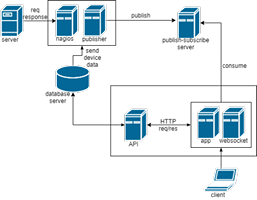
\includegraphics[width=9cm,height=8cm]{assets/images/diagram-arsi.png}
	\caption{Desain Umum Sistem}
	\label{fig:arsiumum}
\end{figure}


\subsection{Desain \textit{Publisher Server}}
Pada \textit{publisher server}, Nagios dipasang untuk memantau keadaan kinerja dari suatu \textit{server}. Kemudian, dipasang pula NRPE untuk mengeksekusi \textit{plugin} Nagios dari jauh. Alasan utama menggunakan NRPE ini adalah memungkinkan Nagios untuk memantau sumber daya "lokal" (seperti beban CPU, penggunaan memori, dan sebagainya). NRPE ini diaplikasikan dengan check-nrpe.

Setiap \textit{server} yang dipantau dimasukkan ke sebuah \textit{thread} baru agar dapat berjalan secara paralel. Kemudian, pada \textit{thread} tersebut setiap \textit{server} terkait akan diperiksa kinerjanya dengan NRPE. Hasil dari pemeriksaan dikirim ke \textit{publish-subscribe server} melalui sebuah \textit{exchange} yang telah diikat dengan sebuah \textit{message queue} yang sudah diinisiasi sebelumnya. Desain dari \textit{publisher server} digambarkan pada Gambar \ref{fig:publisher}

\begin{figure}[H]
	\centering
	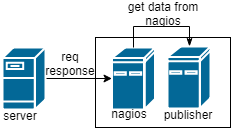
\includegraphics[width=9cm,height=8cm]{assets/images/publisher.png}
	\caption{Desain Publisher Server}
	\label{fig:publisher}
\end{figure}


\subsection{Desain \textit{Publish-Subscribe Server}}
\textit{Publish-subscribe server} adalah sebuah \textit{server} yang berfungsi sebagai wadah untuk menampung pesan dari \textit{publisher} yang mengirimkan data hasil pemantauan oleh Nagios. Pada \textit{server} ini terpasang Rabbitmq sebagai \textit{message broker}. Seluruh pesan yang dikirimkan oleh publisher ditampung ke \textit{publish -subscribe server} melalui sebuah \textit{exchange} yang diikat dengan sebuah \textit{queue}. Setelah itu, \textit{server} akan menyimpan pesan dalam \textit{queue} tersebut hingga ada konsumen, yakni \textit{websocket server}, yang meminta data tersebut untuk dikirimkan.

Secara umum, desain dari \textit{Publish-Subscribe Server} dapat
dilihat pada Gambar \ref{fig:pubsub}.

\begin{figure}[H]
	\centering
	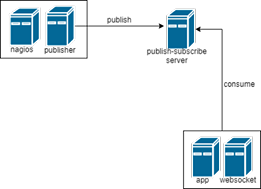
\includegraphics[width=9cm,height=8cm]{assets/images/pubsub.png}
	\caption{Desain Publish-Subscribe Server}
	\label{fig:pubsub}
\end{figure}

\subsection{Desain Webserver}
Pada server ini, terdapat \textit{application server} dan \textit{websocket}. \textit{Websocket} digunakan untuk mengambil data yang dikirimkan oleh \textit{publisher}. Istilahnya, \textit{websocket} ini bertindak sebagai konsumen oleh klien. Data yang diterima sifatnya \textit{realtime} yang berarti merupakan data-data terbaru. 

Konsumen akan membuat sebuah \textit{queue} dengan nama yang ditentukan oleh klien. Nama dari \textit{queue} tersebut ditentukan dengan membuat \textit{string} UUID versi 4 secara acak. Setelah \textit{queue} berhasil dibuat, konsumen membuat \textit{exchange}. Jumlah \textit{exchange} yang terbuat sama banyaknya dengan jumlah \textit{server} yang terdaftar di sistem. Penamaan \textit{exchange} disesuaikan dengan ID masing-masing \textit{server} yang juga berformat UUID versi 4. 

Pembuatan \textit{queue} dan \textit{exchange} ini dilakukan jika \textit{queue} dan \textit{exchange} belum terdaftar pada \textit{publish-subscribe server}. Jika sudah terdaftar, maka tidak dilakukan pembuatan \textit{queue} dan \textit{exchange} lagi. Setelah \textit{queue} dan \textit{exchange} terbuat, maka dilakukan pengikatan (\textit{binding}) \textit{queue} oleh \textit{exchange}. \textit{Queue} dapat diikat oleh satu atau lebih \textit{exchange}. 

Selain itu, semua fitur selain memantau \textit{server} diaplikasikan di \textit{application server}. Fitur-fitur tersebut adalah:
\begin{itemize}
	\item memasukkan data perangkat beserta \textit{service}-nya,
	\item mengubah data perangkat,
	\item menghapus perangkat,
	\item melakukan \textit{subscribe} pada perangkat yang dipilih,
	\item melakukan \textit{unsubscribe}
\end{itemize}


\subsection{Desain \textit{Database Server}}
Desain \textit{database} pada sistem ini adalah seperti yang digambarkan pada Gambar \ref{fig:pdm} di bawah ini. 

\begin{figure}[H]
	\centering
	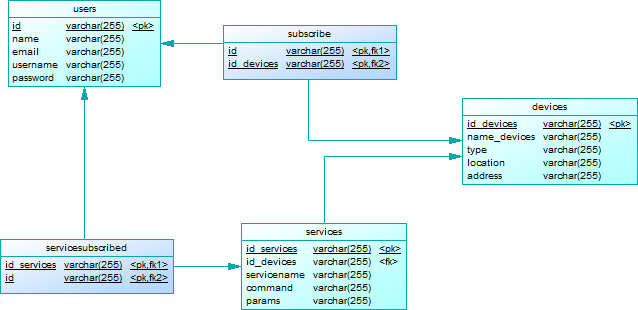
\includegraphics[width=9cm,height=8cm]{assets/images/pdm.png}
	\caption{Physical Data Model}
	\label{fig:pdm}
\end{figure}

Terdapat 5 (lima) tabel pada \textit{database} ini. 3 (tiga) tabel di antaranya adalah tabel berentitas kuat dan merupakan tabel utama pada sistem ini, yaitu: users, devices, dan services. 2 (dua) tabel lainnya merupakan tabel hasil dari relasi \textit{many-to-many}, yaitu tabel subscribe dan servicesubscribe. 

Tabel subscribe ini digunakan untuk menyimpan data pengguna yang melakukan \textit{subscribe} ke suatu \textit{server}. Dan pengguna juga dapat melakukan \textit{subscribe} ke \textit{service} yang dimiliki oleh \textit{server}. \textit{Service} ini berguna untuk mengetahui informasi apa saja yang ada pada tiap perangkat. Tiap \textit{service} memiliki \textit{command} yang berbeda.

\subsection{Desain REST API}
REST API merupakan implementasi dari API (\textit{Application Programming Interface}). REST (\textit{Representional State Transfer}) sendiri adalah suatu arsitektur metode komunikasi yang menggunakan protokol HTTP untuk pertukaran data. Metode ini sering diterapkan dalam pengembangan aplikasi. Tujuan dari REST API yang diterapkan pada pengembangan aplikasi adalah agar sistem memiliki performa yang cepat namun berjalan dengan baik. Sistem juga menjadi mudah dikembangkan terutama dalam hal pertukaran dan komunikasi data. 

URL pada API biasa disebut \textit{endpoint}. Pada sistem ini, terdapat beberapa \textit{endpoint} yang mana masing-masing \textit{endpoint} memiliki \textit{endpoint-endpoint} lagi. 

\textit{Application server} mengirimkan HTTP \textit{request} ke API. Kemudian, API akan melakukan transaksi dengan \textit{database}. Setelah mendapatkan data, maka API akan mengirimkan HTTP \textit{response} ke \textit{application server}. 

Desain dari REST API dapat dilihat pada Gambar \ref{fig:api}. 

\begin{figure}[H]
	\centering
	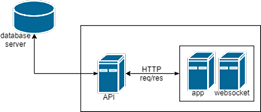
\includegraphics[scale=0.75]{assets/images/rest-api.png}
	\caption{Desain Umum Sistem}
	\label{fig:api}
\end{figure}
	\chapter{IMPLEMENTASI}
\label{chapter:implementasi}

Pada bab ini dijelaskan mengenai implementasi \textit{publish-subscribe} pada rancang bangun sistem \textit{monitoring} perangkat di DPTSI ITS.

\section{Lingkungan Implementasi}
Lingkungan implementasi dalam pembuatan Tugas Akhir ini meliputi perangkat keras dan perangkat lunak yang digunakan untuk rancang bangun sistem \textit{monitoring} perangkat di DPTSI ITS dengan implementasi \textit{publish-subscribe} adalah sebagai berikut:

\begin{enumerate}
	\item Perangkat Keras:
	\begin{itemize}
		\item \textit{Processor} Intel(R) Core(TM) i5-4210U CPU @1.70GHz 64-bit dengan memori RAM 4 GB.
	\end{itemize}
	\item Perangkat Lunak:
	\begin{itemize}
		\item Sistem operasi Ubuntu 14.04 LTS 64 bit.
		\item Rabbitmq, digunakan sebagai broker pada \textit{publish-subscribe}.
		\item Flask, digunakan untuk membuat aplikasi sistem.
		\item Nagios, digunakan untuk memantau server.
		\item MySQL, digunakan untuk membangun \textit{database} pada sistem.
		\item Telegram, digunakan sebagai media penerimaan notifikasi dari sistem.
		\item \textit{Text editor} Sublime Text 3.
		\item TeXstudio, digunakan untuk menyusun buku tugas akhir ini.
		
	\end{itemize}
\end{numerate}
	
\section{Implementasi \textit{Publisher Server}}
	\textit{Publisher server} merupakan \textit{server} yang berfungsi untuk mengambil data pada perangkat (\textit{server}) dan mengirimkannya menuju \textit{publish-subscribe server}. \textit{Publisher server} menggunakan \textit{plugin} NRPE sebagai tambahan pada Nagios untuk memantau sumber daya "lokal" (seperti beban CPU, penggunaan memori, dan sebagainya). Untuk itu kita perlu memasang Nagios terlebih dahulu pada \textit{server} agar bisa melakukan pengambilan data pemantauan \textit{server}. 
	
	Setelah data berhasil dikumpulkan, data hasil pemantauan pada tiap \textit{server} dikirimkan menuju \textit{publish-subscribe server} melalui \textit{thread} yang berbeda. Proses ini dinamakan \textit{multithreading}.
	
	\subsection{Instalasi Nagios pada \textit{Server}}
	Instalasi dilakukan dengan mengunduh Nagios terlebih dahulu pada laman di bawah ini
	\url{https://assets.nagios.com/downloads/nagioscore/releases/nagios-4.3.4.tar.gz}.
	Setelah itu, dilakukan prosedur penginstalan Nagios di \textit{server}.
	
	\subsection{\textit{Script} NRPE untuk Pengambilan Data}
	Kode Sumber \ref{nrpe} ini menunjukkan \textit{script} dari \textit{[plugin]} NRPE untuk megambil data dari hasil pemantauan oleh Nagios.
	
\begin{lstlisting}[frame=single,breaklines,caption={Perintah Mengumpulkan Data Perangkat dengan NRPE},label=nrpe, captionpos=b]
$ /usr/local/nagios/libexec/check_nrpe -H <alamat_server> -c <nama_service> ['nama_command']
\end{lstlisting} 
	
	
	\section{Implementasi \textit{Publish-Subscribe Server}}
	Pada \textit{publish-subscribe server}, dipasang aplikasi RabbitMQ. RabbitMQ menerima seluruh data yang dikirim oleh \textit{publisher}. Setelah itu, RabbitMQ
	menyimpan dan menunggu hingga ada konsumen yang
	meminta data tersebut pada RabbitMQ . Data yang dikirimkan harus sesuai dengan apa yang diminta oleh konsumen, tidak boleh berbeda dari kriteria yang diminta. 
	
	Instalasi RabbitMQ dapat dilihat melalui halaman web resminya, \url{https://www.rabbitmq.com/install-debian.html}. Langkah instalasi diawali dengan penginstalan erlang, sebuah bahasa pemrograman yang dibutuhkan untuk menjalankan RabbitMQ. Setelah itu barulah dipasang \texttt{rabbitmq-server}. 
	
	Setelah RabbitMQ \textit{server} terpasang, selanjutnya dilakukan konfigurasi untuk mengaktifkan akses ke RabbitMQ Management Console, web admin milik RabbitMQ. Hal ini dilakukan agar mudah untuk melakukan manajemen data, \textit{user}, dan lain-lain. RabbitMQ sudah menyediakan \textit{plugin} agar web admin dapat langsung digunakan. Hanya dengan menjalankan perintah \texttt{sudo rabbitmq-plugins enable rabbitmq\_management}, web admin RabbitMQ dapat dijalankan. 
	
	\section{Implementasi \textit{Webserver}}
	Pada \textit{webserver}, terdapat \textit{application server} dan \textit{websocket.} \textit{Websocket} berfungsi untuk meminta data dari \textit{publish-subscribe server}. Websocket disambungkan dengan suatu \textit{endpoint} pada \textit{application server}, sehingga ketika klien mengakses \textit{endpoint} pada aplikasi, \texttt{javascript} pada halaman tersebut akan menyambungkan ke halaman pada \textit{websocket}.
	
	\textit{Websocket} pada sistem ini menggunakan node.js, sebuah perangkat lunak yang didesain untuk mengembangkan aplikasi berbasis web. Node.js menggunakan bahasa pemrograman JavaScript.\\
	
	\begin{lstlisting}[frame=single,caption={Inisiasi Komunikasi Websocket dengan Klien dan Publish-Subscribe Server Tidak Terkonesi}, breaklines=true,label=pseudo:notconn, language=python]
	socket.on('disconnect', function() {
	$("#idlogs").text("Disconnect");
	$("#idlogs").parent().parent().attr('class', 'block-content block-content-full bg-danger');
	$('.nrperesult').each(function() {
	$(this).html("")
	});
	});
	\end{lstlisting}
	
	Kode Sumber \ref{pseudo:notconn} menunjukkan jika kondisi komunikasi antara \textit{websocket} dengan klien dan \textit{publish-subscribe server} tidak tersambung.
	
	\begin{lstlisting}[frame=single,caption={Inisiasi Komunikasi Websocket dengan Klien dan Publish-Subscribe Server Terkoneksi}, breaklines=true,label=pseudo:conn, language=python]
	socket.on('connect', function() {
	$("#idlogs").text("Connected");
	$("#idlogs").parent().parent().attr('class', 'block-content block-content-full bg-success');
	
	var deviceid = [];
	$('.device').each(function( index ) {
	deviceid.push($( this ).attr('id'));
	});
	socket.emit('startRabbit', {'data': deviceid, 'id': uuid4() });
	
	});
	\end{lstlisting}
	
	Kode Sumber \ref{pseudo:conn} menunjukkan jika kondisi komunikasi antara \textit{websocket} dengan klien dan \textit{publish-subscribe server} telah tersambung. Kemudian, klien mengirimkan ID dari perangkat (\textit{server}) yang telah dipilih oleh pengguna untuk menjadikannya nama \textit{exchange}. UUID versi 4 dibuat untuk menamai \textit{queue} yang baru. 
	
	Jika koneksi sudah tersambung dan ID perangkat untuk penamaan \textit{exchange} serta UUID versi 4 untuk penamaan \textit{queue} sudah dikirim oleh klien, maka selanjutnya \textit{server} akan memproses pembuatan \textit{exchange} dan \textit{queue} baru. Kode \textit{websocket server} saat pembuatan
	\textit{exchange} dan \textit{queue} lalu menyalurkan data pada klien dapat dilihat pada Kode Sumber \ref{pseudo:buatbaru}
	
\begin{lstlisting}[frame=single,caption={Pembuatan Exchange dan Queue Baru pada Websocket}, breaklines=true,label=pseudo:buatbaru, language=python]
rabbitMqConnection.createChannel().then(function(ch) {
consumerChannel = ch
var q;
function allDone(notAborted, arr) {
var okok = ch.prefetch(1)
okok = okok.then(() => {
return ch.consume(q, logMessage, {noAck: true}) 
.then(() => {
console.log(' [*] Waiting for '+msg['data']+'.');
})
})
}
forEach(msg['data'], function (item, index, arr) {
var done = this.async()
var ok = ch.assertExchange(item, 'fanout', {durable: false});
ok = ok.then(function() {
return ch.assertQueue(msg['id'], {exclusive: false});
});
ok = ok.then(function(qok) {
return ch.bindQueue(qok.queue, item, '').then(function() {
q = qok.queue
return qok.queue;
});
});
ok = ok.then(function() {
done()
})
}, allDone)
\end{lstlisting}
	
	\section{Implementasi REST API}
	Fungsi utama dari REST API untuk sistem ini adalah untuk menyimpan data pengguna yang melakukan \textit{subscribe} pada perangkat beserta \textit{service}-nya. REST API dibuat dengan menggunakan \textit{framework} Flask dan ORM Database peewee.
	
	REST API menggunakan protokol HTTP dalam pengaksesannya. Sehingga, terdapat URL API yang dapat disebut sebagai \textit{endpoint}. Tabel \ref{tab:endpoint} akan menguraikan ada \textit{endpoint} apa saja pada REST API di sistem ini. 
	
	\begin{longtable}{|p{0.05\textwidth}|p{0.40\textwidth}|p{0.13\textwidth}|p{0.25\textwidth}|} % L = Rata kiri untuk setiap kolom, | = garis batas vertikal.
		
		% Kepala tabel, berulang di setiap halaman
		\caption{Daftar Endpoint pada REST API} \label{tab:endpoint} \\
		\hline
		\textbf{No} & \textbf{\textit{Endpoint}} & \textbf{Metode} & \textbf{Aksi} \\ \hline
		\endhead
		\endfoot
		\endlastfoot
		1 & /register & POST & Membuat data baru pada tabel user di database \\ \hline
		2 & /login & POST & Mengambil data pada tabel user dan mencocokkannya dengan JSON yang dikirimkan lewat \textit{body}. setelah data username dan password cocok, lalu dibuatkan sebuah token JWT. \\ \hline
		3 & /logout & POST & Memasukkan token JWT yang terdaftar pada server kedalam daftar hitam agar token tidak dapat digunakan lagi. \\ \hline
		4 & /users & GET & Menampilkan seluruh data user yang terdaftar pada sistem \\ \hline
		5 & /users/\textless{}string:username\textgreater{} & GET & Menampilkan data user berdasarkan username yang tertulis pada URL \\ \hline
		6 & /devices/create & POST & Membuat data baru pada tabel devices di database \\ \hline
		7 & /devices/edit/\textless{}string:id\textgreater{} & PUT & Mengubah data pada tabel devices di database yang ID nya sama dengan ID yang ada pada URL. \\ \hline
		8 & /devices/delete & DELETE & Menghapus data pada tabel devices di database yang ID nya tertulis pada \textit{body} yang bertipe JSON. \\ \hline
		9 & /devices & GET & Menampilkan seluruh data perangkat yang terdaftar pada sistem \\ \hline
		10 & /devices/\textless{}string:id\textgreater{} & GET & Menampilkan data user berdasarkan username yang tertulis pada URL \\ \hline
		11 & /service/create & POST & Membuat data baru pada tabel service \\ \hline
		12 & /service/edit & POST & Mengubah data pada tabel service di database yang ID nya tertulis pada \textit{body} yang bertipe JSON. \\ \hline
		13 & /service/delete & POST & Menghapus data pada tabel service di database yang ID nya tertulis pada \textit{body} yang bertipe JSON. \\ \hline
		14 & /subscribe/devices & POST & Membuat data baru pada tabel subscribe \\ \hline
		15 & /unsubscribe/devices & POST & Menghapus data pada tabel subscribe di database yang ID nya tertulis pada \textit{body} yang bertipe JSON. \\ \hline
		16 & /subscribe/service & POST & Membuat data baru pada tabel servicesubscribed \\ \hline
		17 & /unsubscribe/service & POST & Menghapus data pada tabel servicesubscribed di database yang ID nya tertulis pada \textit{body} yang bertipe JSON. \\ \hline	
	\end{longtable}
	


	\chapter{PENGUJIAN DAN EVALUASI}
	Pada bab ini akan dibahas uji coba dan evaluasi dari sistem yang telah dibuat. Sistem akan diuji coba fungsionalitas dan performanya dengan menjalankan skenario uji coba yang sudah ditentukan. Uji coba dilakukan untuk mengetahui hasil dari sistem ini sehingga dapat menjawab rumusan masalah pada tugas akhir ini.    
	
\section{Lingkungan Uji Coba}
	Lingkungan pengujian menggunakan komponen-komponen yang terdiri dari: satu \textit{server publisher}, satu \textit{server publish-subscribe}, satu \textit{server} aplikasi dan API, satu \textit{server database}, dan satu komputer penguji. Pengujian dilakukan di Laboratoriom Arsitektur dan Jaringan Komputer Departemen Informatika ITS. \\
    \indent Spesifikasi untuk setiap komponen yang digunakan ditunjukkan pada Tabel \ref{spesifikasipublisher} untuk \textit{publisher server}, Tabel \ref{spesifikasipubsub} untuk \textit{publish-subscribe server}, Tabel \ref{spekwebserver} untuk \textit{web server} dan API, Tabel \ref{spekdbserver} untuk \textit{database server}, dan Tabel \ref{spesifikasikomputerpenguji} untuk komputer penguji.
\pagebreak
\begin{enumerate}
	\item \textbf{\textit{Publisher Server}}
	\begin{longtable}{|l|l|}
		\caption{\textit{Server} Untuk \textit{Publisher}}
		\label{spesifikasipublisher} \\
		\hline
		\textbf{Perangkat Keras}      & \begin{tabular}[c]{@{}l@{}} Processor Intel(R) Core(TM) \\ i5-2120 CPU @ 3.30GHz\end{tabular} \\ \cline{2-2} 
		& RAM 8GB	\\ \cline{2-2} 
		& Hard disk 500GB \\ \hline
		\textbf{Perangkat Lunak}      & Ubuntu 16.04 64 bit \\ \cline{2-2} 
		& Nagios \\ \hline
		\textbf{Konfigurasi Jaringan} & IP address : 10.151.36.97 \\ \cline{2-2} 
		& Netmask : 255.255.255.0 \\ \cline{2-2} 
		& Gateway : 10.151.36.1 \\ \hline
	\end{longtable}
	
	\item \textbf{\textit{Publish-Subscribe Server}}
	\begin{longtable}{|l|l|}
		\caption{\textit{Server} Untuk \textit{Publish-Subscribe}}
		\label{spesifikasipubsub} \\
		\hline
		\textbf{Perangkat Keras}      & \begin{tabular}[c]{@{}l@{}} Processor Intel(R) Core(TM) \\ i5-2120 CPU @ 3.30GHz\end{tabular} \\ \cline{2-2} 
		& RAM 8GB	\\ \cline{2-2} 
		& Hard disk 500GB \\ \hline
		\textbf{Perangkat Lunak}      & Ubuntu 16.04 64 bit \\ \cline{2-2} 
		& RabbitMQ \\ \hline
		\textbf{Konfigurasi Jaringan} & IP address : 10.151.36.70 \\ \cline{2-2} 
		& Netmask : 255.255.255.0 \\ \cline{2-2} 
		& Gateway : 10.151.36.1 \\ \hline
	\end{longtable}

	\item \textbf{\textit{Web Server} dan API}
	\begin{longtable}{|l|l|}
		\caption{\textit{Server} Untuk Aplikasi dan API}
		\label{spekwebserver} \\
		\hline
		\textbf{Perangkat Keras}      & \begin{tabular}[c]{@{}l@{}} Processor Intel(R) Core(TM) \\ i5-2120 CPU @ 3.30GHz\end{tabular} \\ \cline{2-2} 
		& RAM 8GB	\\ \cline{2-2} 
		& Hard disk 500GB \\ \hline
		\textbf{Perangkat Lunak}      & Ubuntu 14.04 64 bit \\ \cline{2-2} 
		& RabbitMQ \\ \cline{2-2}
		& Flask \\ \cline{2-2}
		& NodeJS \\ \hline
		\textbf{Konfigurasi Jaringan} & IP address : 10.151.36.33 \\ \cline{2-2} 
		& Netmask : 255.255.255.0 \\ \cline{2-2} 
		& Gateway : 10.151.36.1 \\ \hline
	\end{longtable}

	\item \textbf{\textit{Database Server}}
	\begin{longtable}{|l|l|}
		\caption{\textit{Server} Untuk \textit{Database}}
		\label{spekdbserver} \\
		\hline
		\textbf{Perangkat Keras}      & \begin{tabular}[c]{@{}l@{}} Processor Intel(R) Core(TM) \\ i5-2120 CPU @ 3.30GHz\end{tabular} \\ \cline{2-2} 
		& RAM 8GB	\\ \cline{2-2} 
		& Hard disk 500GB \\ \hline
		\textbf{Perangkat Lunak}      & Ubuntu 16.04 64 bit \\ \cline{2-2} 
		& MySQL Server \\ \hline
		\textbf{Konfigurasi Jaringan} & IP address : 10.151.36.101 \\ \cline{2-2} 
		& Netmask : 255.255.255.0 \\ \cline{2-2} 
		& Gateway : 10.151.36.1 \\ \hline
	\end{longtable}
		
	\item \textbf{Komputer Penguji}
	\begin{longtable}{|l|l|}
		\caption{Komputer Penguji}
		\label{spesifikasikomputerpenguji} \\
		\hline
		\textbf{Perangkat Keras}      & \begin{tabular}[c]{@{}l@{}} Processor Intel(R) Core(TM) \\ i5-2120 CPU @ 3.30GHz\end{tabular} \\ \cline{2-2} 
		& RAM 8GB	\\ \cline{2-2} 
		& Hard disk 500GB \\ \hline
		\textbf{Perangkat Lunak}      & Ubuntu 14.04 64 bit \\ \cline{2-2} 
		& Google Chrome \\ \hline
		\textbf{Konfigurasi Jaringan} & IP address : 10.151.36.33 \\ \cline{2-2} 
		& Netmask : 255.255.255.0 \\ \cline{2-2} 
		& Gateway : 10.151.36.1 \\ \hline
	\end{longtable}

\end{enumerate}
			
   
\section{Skenario Uji Coba} \label{skenarioujicoba}
	Uji coba akan dilakukan untuk mengetahui keberhasilan sistem yang telah dibangun. Skenario pengujian dibedakan menjadi 2 bagian, yaitu:
    \begin{itemize}
    \item \textbf{Uji Fungsionalitas} \\
    	Pengujian ini didasarkan pada fungsionalitas yang disajikan sistem.
    \item \textbf{Uji Performa} \\
    	Pengujian ini untuk menguji ketahanan sistem terhadap sejumlah permintaan ke aplikasi secara bersamaan.
    \end{itemize}
    
\subsection{Skenario Uji Coba Fungsionalitas}
Uji coba fungsionalitas dilakukan dengan cara menjalankan sistem yang telah dibangun dan melakukan pengujian terhadap fitur yang telah dibuat. Uji coba fungsionalitas akan berfungsi untuk memastikan sistem sudah memenuhi kebutuhan.

\subsubsection{Uji Pengguna Dapat Melihat Data Perangkat} \label{pertama}
Pengujian ini dilakukan untuk mengetahui apakah pengguna dapat melihat data perangkat yang telah terdaftar di sistem.

Pengujian dilakukan setelah pengguna melakukan \textit{login}. Uji fungsionalitas pengguna dapat melihat data perangkat yang telah terdaftar di sistem dijelaskan pada Tabel \ref{lihatperangkat}.
\begin{longtable}{|p{0.05\textwidth}|p{0.38\textwidth}|p{0.39\textwidth}|}					\caption{Skenario Uji Pengguna Dapat Melihat Data Perangkat} \label{lihatperangkat} \\
	\hline
	\textbf{No} & \textbf{Uji Coba} & \textbf{Hasil Harapan} \\ \hline
	\endfirsthead
	\caption[]{Skenario Uji Melihat Data Perangkat} \\
	\hline
	\textbf{No} & \textbf{Uji Coba} & \textbf{Hasil Harapan} \\ \hline
	\endhead
	\endfoot
	\endlastfoot
	
	1 & Pengguna menekan tombol menu 'Device Management'. & Pengguna dapat melihat perangkat apa saja yang terdaftar di sistem.\\ \hline
\end{longtable}

\paragraph{Uji Pengguna Dapat Melihat Detail Data Perangkat} \label{kedua}
Pengujian ini dilakukan untuk mengetahui apakah pengguna dapat melihat rincian data dari suatu perangkat.

Uji fungsionalitas pengguna dapat melihat detail data perangkat yang telah terdaftar di sistem dijelaskan pada Tabel \ref{lihatdetilperangkat}.

\begin{longtable}{|p{0.05\textwidth}|p{0.38\textwidth}|p{0.39\textwidth}|}					\caption{Skenario Uji Pengguna Dapat Melihat Detail Data Perangkat} \label{lihatdetilperangkat} \\
	\hline
	\textbf{No} & \textbf{Uji Coba} & \textbf{Hasil Harapan} \\ \hline
	\endfirsthead
	\caption[]{Skenario Uji Melihat Detail Data Perangkat} \\
	\hline
	\textbf{No} & \textbf{Uji Coba} & \textbf{Hasil Harapan} \\ \hline
	\endhead
	\endfoot
	\endlastfoot
	
	1 & Pengguna menekan tombol menu 'Info' yang ada pada tiap perangkat. & Pengguna dapat melihat detail data dari suatu perangkat.\\ \hline
\end{longtable}

\paragraph{Uji Pengguna Dapat Mengubah Data Perangkat} \label{ketiga}
Pengujian ini dilakukan untuk mengetahui apakah pengguna dapat mengubah data dari suatu perangkat.

Uji fungsionalitas pengguna dapat mengubah data perangkat dijelaskan pada Tabel \ref{ubahdata}

\begin{longtable}{|p{0.05\textwidth}|p{0.38\textwidth}|p{0.39\textwidth}|}					\caption{Skenario Uji Pengguna Dapat Mengubah Data Perangkat} \label{ubahdata} \\
	\hline
	\textbf{No} & \textbf{Uji Coba} & \textbf{Hasil Harapan} \\ \hline
	\endfirsthead
	\caption[]{Skenario Uji Pengguna Dapat Mengubah Data Perangkat} \\
	\hline
	\textbf{No} & \textbf{Uji Coba} & \textbf{Hasil Harapan} \\ \hline
	\endhead
	\endfoot
	\endlastfoot
	
	1 & Pengguna menekan tombol menu 'Ubah' yang ada pada tiap perangkat. & Sistem menampilkan \textit{form} yang sudah berisi detail data dari perangkat.\\ \hline
	2 & Pengguna mengubah data perangkat sesuai kebutuhan. & Sistem menampilkan data yang sudah diubah oleh pengguna sebelumnya menggantikan data yang lama. \\ \hline
\end{longtable}

\paragraph{Uji Pengguna Dapat Menghapus Data Perangkat} \label{keempat}
Pengujian ini dilakukan untuk mengetahui apakah pengguna dapat menghapus data perangkat dari sistem.

Uji fungsionalitas pengguna dapat menghapus data perangkat dari sistem dijelaskan pada Tabel \ref{hapusdata}.

\begin{longtable}{|p{0.05\textwidth}|p{0.38\textwidth}|p{0.39\textwidth}|}					\caption{Skenario Uji Pengguna Dapat Menghapus Data Perangkat} \label{hapusdata} \\
	\hline
	\textbf{No} & \textbf{Uji Coba} & \textbf{Hasil Harapan} \\ \hline
	\endfirsthead
	\caption[]{Skenario Uji Menghapus Data Perangkat} \\
	\hline
	\textbf{No} & \textbf{Uji Coba} & \textbf{Hasil Harapan} \\ \hline
	\endhead
	\endfoot
	\endlastfoot
	
	1 & Pengguna menekan tombol menu 'Hapus' yang tersedia pada tiap perangkat. & Data perangkat berhasil dihapus.\\ \hline
\end{longtable}

\subsubsection{Uji Pengguna Dapat Melakukan \textit{Subscribe} pada Perangkat} \label{kelima}
Pengujian ini dilakukan untuk mengetahui apakah pengguna dapat melakukan \textit{subscribe} pada perangkat yang dipilih. 

Uji fungsionalitas pengguna dapat melakukan \textit{subscribe} pada perangkat yang dipilih dijelaskan pada Tabel \ref{subscribe}.

\begin{longtable}{|p{0.05\textwidth}|p{0.38\textwidth}|p{0.39\textwidth}|}					\caption{Skenario Uji Pengguna Dapat Melakukan \textit{Subscribe} pada Perangkat} \label{subscribe} \\
	\hline
	\textbf{No} & \textbf{Uji Coba} & \textbf{Hasil Harapan} \\ \hline
	\endfirsthead
	\caption[]{Skenario Uji Melakukan \textit{Subscribe} pada Perangkat} \\
	\hline
	\textbf{No} & \textbf{Uji Coba} & \textbf{Hasil Harapan} \\ \hline
	\endhead
	\endfoot
	\endlastfoot
	
	1 & Pengguna menekan tombol 'Subscribe' yang tersedia pada tiap perangkat. & Pengguna berhasil melakukan \textit{subscribe} pada perangkat yang telah dipilih ditandai dengan berubahnya tombol 'Subscribe' menjadi 'Unsubscribe'.\\ \hline
\end{longtable}

\subsubsection{Uji Pengguna Dapat Menghentikan \textit{Subscribe} (\textit{Unsubscribe}) pada Perangkat} \label{keenam}
Pengujian ini dilakukan untuk mengetahui apakah pengguna dapat berhenti langganan dari perangkat yang dipilih sebelumnya. 

Uji fungsionalitas pengguna dapat melakukan \textit{unsubscribe} pada perangkat yang dipilih sebelumnya dijelaskan pada Tabel \ref{unsubscribe}.

\begin{longtable}{|p{0.05\textwidth}|p{0.38\textwidth}|p{0.39\textwidth}|}					\caption{Skenario Uji Pengguna Dapat Menghentikan \textit{Subscribe} (\textit{Unsubscribe}) pada Perangkat} \label{usubscribe} \\
	\hline
	\textbf{No} & \textbf{Uji Coba} & \textbf{Hasil Harapan} \\ \hline
	\endfirsthead
	\caption[]{Skenario Uji Menghentikan \textit{Subscribe} (\textit{Unsubscribe}) pada Perangkat} \\
	\hline
	\textbf{No} & \textbf{Uji Coba} & \textbf{Hasil Harapan} \\ \hline
	\endhead
	\endfoot
	\endlastfoot
	
	1 & Pengguna menekan tombol 'Unsubscribe' yang tersedia pada tiap perangkat yang sebelumnya di-\textit{subscribe}. & Pengguna berhasil melakukan \textit{unsubscribe} pada perangkat yang ditandai dengan berubahnya tombol 'Unsubscribe' menjadi 'Subscribe' kembali.\\ \hline
\end{longtable}

\subsubsection{Uji Pengguna Dapat Melakukan \textit{Monitoring} atau Pemantauan pada Perangkat yang Telah Di-\textit{Subscribe}} \label{ketujuh}
Pengujian ini dilakukan untuk mengetahui apakah pengguna dapat memantau perangkat yang di-\textit{subscribe} sebelumnya. 

Uji fungsionalitas pengguna dapat melakukan \textit{monitoring} atau pemantauan pada perangkat yang di-\textit{subscribe} sebelumnya dijelaskan pada Tabel \ref{monitor}.

\begin{longtable}{|p{0.05\textwidth}|p{0.38\textwidth}|p{0.39\textwidth}|}					\caption{Skenario Uji Pengguna Dapat Melakukan \textit{Monitoring} atau Pemantauan pada Perangkat yang Telah Di-\textit{Subscribe}} \label{monitor} \\
	\hline
	\textbf{No} & \textbf{Uji Coba} & \textbf{Hasil Harapan} \\ \hline
	\endfirsthead
	\caption[]{Skenario Uji Melakukan \textit{Monitoring} atau Pemantauan pada Perangkat yang Telah Di-\textit{Subscribe}} \\
	\hline
	\textbf{No} & \textbf{Uji Coba} & \textbf{Hasil Harapan} \\ \hline
	\endhead
	\endfoot
	\endlastfoot
	
	1 & Pengguna menekan tombol menu 'Monitor' yang tersedia di sistem. & Pengguna dapat melihat kondisi perangkat yang di-\textit{subscribe}.\\ \hline
\end{longtable}

\subsection{Skenario Uji Coba Performa}
Uji performa dilakukan dengan dua skenario, yaitu uji performa REST API dan uji performa \textit{publish-subscribe}. Uji coba REST API dilakukan dengan menggunakan satu buah komputer untuk melakukan akses secara bersamaan ke REST API menggunakan bantuan aplikasi JMeter, sebuah aplikasi pengujian untuk menganalisa dan menghitung performa dari suatu servis.

Sedangkan untuk uji performa \textit{publish-subscribe} dilakukan dengan cara menghitung waktu pengiriman data. Data dikirim oleh publisher yang berada pada server dengan alamat IP 10.151.36.97 menuju konsumen yang berada pada alamat IP 10.151.36.33.

\subsubsection{Uji Performa REST API}
Pengujian dilakukan menggunakan bantuan aplikasi JMeter untuk mengukur jumlah waktu yang diperlukan oleh REST API untuk menyelesaikan \textit{request} dari komputer penguji.

\subsubsection{Uji Performa \textit{Publish-Subscribe}}
Pengujian dilakukan dengan mengukur jumlah waktu yang diperlukan \textit{publisher} dalam mengirim data dan diterima oleh \textit{subscriber}.

    
\section{Hasil Uji Coba dan Evaluasi}
Berikut dijelaskan hasil uji coba dan evaluasi berdasarkan skenario yang telah dijelaskan pada subbab \ref{skenarioujicoba}.
    
\subsection{Uji Fungsionalitas}
Berikut dijelaskan hasil pengujian fungsionalitas pada sistem yang dibangun.

\subsubsection{Uji Pengguna Dapat Melihat Data Perangkat}
Pengujian dilakukan sesuai dengan skenario yang dijelaskan pada subbab \ref{pertama} dan pada Tabel \ref{lihatperangkat}. Hasil pengujian pengguna melihat data perangkat yang telah terdaftar di sistem dapat dilihat pada Tabel \ref{hasilpertama}

\begin{longtable}{|p{0.05\textwidth}|p{0.55\textwidth}|p{0.22\textwidth}|}					\caption{Hasil Uji Coba \textit{Client} dapat Mengakses Internet} \label{hasilpertama} \\
	\hline
	\textbf{No} & \textbf{Uji Coba} & \textbf{Hasil} \\ \hline
	\endfirsthead
	\caption[]{Hasil Uji Pengguna Melihat Data Perangkat} \\
	\hline
	\textbf{No} & \textbf{Uji Coba} & \textbf{Hasil} \\ \hline
	\endhead
	\endfoot
	\endlastfoot
	
	1 & Pengguna menekan tombol menu 'Device Management'. & Data berhasil ditampilkan. \\ \hline
\end{longtable}

Sesuai dengan skenario uji coba  yang diberikan pada Tabel \ref{lihatperangkat}, hasil uji coba menunjukkan skenario berhasil ditangani.

\subsection{Hasil Uji Performa}
Seperti yang sudah dijelaskan pada subbab \ref{skenarioujicoba} pengujian performa dilakukan dengan menggunakan sebuah komputer yang berperan sebagai klien untuk melakukan \textit{monitoring} terhadap perangkat (\textit{server}). 

\subsubsection{Hasil Uji Coba Performa pada REST API}


\subsubsection{Hasil Uji Coba Performa pada \textit{Publish-Subscribe}}



	\chapter{PENUTUP}
    Bab ini membahas kesimpulan yang dapat diambil dari tujuan pembuatan sistem dan hubungannya dengan hasil uji coba dan evaluasi yang telah dilakukan. Selain itu, terdapat beberapa saran yang bisa dijadikan acuan untuk melakukan pengembangan dan penelitian lebih lanjut.
        
\section{Kesimpulan}
Dari proses perancangan, implementasi dan pengujian terhadap sistem, dapat diambil beberapa kesimpulan berikut:
\begin{enumerate}
\item Sistem dapat mengarahkan \textit{client} ke halaman \textit{login} dari sistem.
\item Sistem dapat membuatkan kontainer \textit{docker} yang berisi \textit{mitmproxy} secara otomatis ketika terdapat \textit{client} yang berhasil \textit{login} ke dalam sistem.
\item Sistem dapat mengarahkan \textit{traffic} dari \textit{client} ke kontainer \textit{docker} yang sudah dibuat dan digunakan sebagai internet \textit{access management} bagi \textit{client} dan memperbolehkan atau mengijinkan \textit{client} tersebut untuk mengakses internet. 
\end{enumerate}

\section{Saran}
Berikut beberapa saran yang diberikan untuk pengembangan lebih lanjut:
\begin{enumerate}
\item Sistem dapat dikembangkan dengan menggunakan \textit{server} lebih dari satu untuk meringankan beban kerja dari \textit{server} itu sendiri.
\item Sistem dapat dikembangkan dengan menentukan beban dari setiap \textit{server}, dengan menambahkan kriteria-kriteria yang sesuai dengan lingkungan sistem yang ada, seperti jarak antara \textit{docker host} dengan \textit{middleware} atau kecepatan bandwith dari setiap \textit{docker host} merupakan kriteria yang baik. 
\end{enumerate}

	\bibliography{Zotero}
	\bibliographystyle{IEEEtranID.bst}
    
    \renewcommand\chaptername{LAMPIRAN}
	\appendix
    \chapter{INSTALASI PERANGKAT LUNAK}

\section*{Instalasi Pustaka Python} \label{install:pythonlibrary}
	Dalam pengembangan sistem ini, digunakan berbagai pustaka pendukung. Pustaka pendukung yang digunakan merupakan pustaka untuk bahasa pemrograman Python. Berikut adalah daftar pustaka yang digunakan dan cara pemasangannya:
    \begin{itemize}
	 \item Python Pip\\
		 \$ \texttt{sudo apt-get install python-pip}
    \item Python Dev \\
    	\$ \texttt{sudo apt-get install python-dev}
    \item Setuptools \\
    	\$ \texttt{sudo apt-get install python-setuptools}
    \item MySQLd \\
    	\$ \texttt{sudo apt-get install python-mysqldb}
    \end{itemize}
	
\section*{Pemasangan kerangka kerja Flask}
Dalam pengembangan sistem ini, digunakan Flask karena Flask merupakan kerangka kerja yang menggunakan bahasa pemrograman Python. Untuk memasang Flask, jalankan perintah \texttt{sudo pip3 install flask}.

\section*{Pemasangan perangkat lunak Gunicorn}
Dalam pengembangan sistem ini, digunakan Gunicorn untuk menangani servis dari halaman \textit{login}. Untuk memasang Gunicorn, jalankan perintah \texttt{sudo pip3 install gunicorn}.

\section*{Pemasangan perangkat lunak Supervisor}
Dalam pengembangan sistem ini, digunakan Supervisor supaya servis pada halaman \textit{login} dapat langsung berjalan ketika \textit{server} dinyalakan. Untuk memasang Supervisor, jalankan perintah \texttt{sudo apt-get install supervisor}.

\section*{Pemasangan perangkat lunak Nginx}
Dalam pengembangan sistem ini, digunakan Nginx sebagai web \textit{server} untuk halaman \textit{login}. Untuk memasang Nginx, jalankan perintah \texttt{sudo apt-get install nginx}.

\section*{Instalasi Lingkungan Docker}
Proses pemasangan Docker dpat dilakukan sesuai tahap berikut:
\begin{itemize}
	\item Menambahkan repository Docker\\
	Langkah ini dilakukan untuk menambahkan \textit{repository} Docker ke dalam paket \texttt{apt} agar dapat di unduh oleh Ubuntu. Untuk melakukannya, jalankan perintah berikut:
	\begin{tabbing}
		\texttt{sudo apt-get -y install \char`\\} \\
		\hspace{5 mm} \texttt{apt-transport-https \char`\\} \\
		\hspace{5 mm} \texttt{ca-certificates \char`\\} \\
		\hspace{5 mm} \texttt{curl} \\
		\\
		\texttt{curl -fsSL https://download.docker.com/linux/} \\
		\hspace{7 mm} \texttt{ubuntu/gpg | sudo apt-key add -} \\
		\\
		\texttt{sudo add-apt-repository \char`\\} \\
		\hspace{7 mm} \texttt{"deb [arch=amd64] https://download.docker.com/} \\
		\hspace{9 mm} \texttt{linux/ubuntu \char`\\} \\
		\hspace{7 mm} \texttt{\$ (lsb\_release -cs) \char`\\} \\
		\hspace{7 mm} \texttt{stable"} \\
		\\
		\texttt{sudo apt-get update} \\
	\end{tabbing}
	
	\item Mengunduh Docker \\
	Docker dikembangkan dalam dua versi, yaitu CE (\textit{Community Edition}) dan EE (\textit{Enterprise Edition}). Dalam pengembangan sistem ini, digunakan Docker CE karena merupakan versi Docker yang gratis. Untuk mengunduh Docker CE, jalankan perintah \texttt{sudo apt-get -y install docker-ce}.
	
	\item Mencoba menjalankan Docker \\
	Untuk melakukan tes apakah Docker sudah terpasang dengan benar, gunakan perintah \texttt{sudo docker run hello-world}.
\end{itemize}
    \chapter{Konfigurasi}

\section*{Konfigurasi Supervisor}

Supaya servis pada halaman \textit{login} dapat langsung berjalan, penulis menambahkan konfigurasi perangkat lunak Supervisor pada \texttt{/etc/supervisor/conf.d/app.conf} sepert pada Kode Sumber \ref{appconf}. 

\begin{lstlisting}[frame=single,tabsize=2,breaklines,caption={Isi Berkas app.conf},label=appconf, captionpos=b]
command = /home/fourirakbar/flask-loginpage/flask-loginpageenv/bin/python /home/fourirakbar/flask-loginpage/flask-loginpageenv/bin/gunicorn -b 0.0.0.0:4000 app:app

directory = /home/fourirakbar/flask-loginpage

user = fourirakbar

stdout_logfile = /home/fourirakbar/flask-loginpage/logs/app_stdout.log

stderr_logfile = /home/fourirakbar/flask-loginpage/logs/app_stderr.log

redirect_stderr = True
autostart = True
enviroment = PATH = "/home/fourirakbar/flask-loginpage/flask-loginpageenv/bin", 

PRODUCTION=1
\end{lstlisting}

Perlu diperhatikan ketika menambahkan atau mengubah konfigurasi Supervisor pada \texttt{/etc/supervisor/conf.d/} yang telah di \textit{server} untuk halaman \textit{login}, perlu dilakukan \textit{reload Supervisor} dengan menjalankan \textit{command} pada terminal seperti pada Kode Sumber \ref{reloadsupervisor}.
\begin{lstlisting}[frame=single,tabsize=2,breaklines,caption=Command untuk Reload Supervisor,language=Python,label=reloadsupervisor,captionpos=b]
sudo supervisorctl reread
sudo supervisorctl reload
sudo supervisorctl status
\end{lstlisting}

Perlu diperhatikan pula ketika menambahkan atau mengubah konfigurasi Nginx pada \texttt{/etc/nginx/sites-available/} yang telah di \textit{server} untuk halaman \textit{login}, perlu dilakukan aktifasi konfigurasi Nginx dengan menjalankan \textit{command} pada terminal seperti pada Kode Sumber \ref{aktifasikonfigurasinginx}.
\begin{lstlisting}[frame=single,tabsize=2,breaklines,caption=Command untuk mengaktifkan konfigurasi Nginx,language=Python,label=aktifasikonfigurasinginx,captionpos=b]
sudo ln -s /etc/nginx/sites-available/app 
/etc/nginx/sites-enabled/app
\end{lstlisting}

Setelah itu, jalankan Kode Sumber \ref{restartnginx} supaya konfigurasi yang baru saja diaktifkan dapat digunakan.\\
\begin{lstlisting}[frame=single,tabsize=2,breaklines,captionpos=b,caption=Command untuk merestart Nginx,language=Python,label=restartnginx]
sudo service nginx restart
\end{lstlisting}

\section*{Konfigurasi Nginx}

Supaya web \textit{server} untuk halaman \textit{login} dapat dijalankan, penulis menambahkan konfigurasi perangkat lunak Nginx pada \texttt{/etc/nginx/sites-available/app} seperti pada Kode Sumber \ref{nginxapp}.

\begin{lstlisting}[frame=single,tabsize=2,breaklines,caption={Isi Berkas app},label=nginxapp, captionpos=b]
server {
	listen 80;
	server_name 10.151.36.173;
	
	add_header X-Frame-Options SAMEORIGIN;
	add_header X-Content-Type-Options nosniff;
	add_header X-XSS-Protection "1; mode=block";
	
	access_log /home/fourirakbar/flask-loginpage/logs/app_access.log;
	location / {
		proxy_pass       http://127.0.0.1:4000;
		proxy_set_header Host        $host;
		proxy_set_header X-Real-IP   $remote_addr;
		proxy_set_header X-Forwarded-For $proxy_add_x_forwarded_for;
	}
	location ^~ /static/  {
	include     /etc/nginx/mime.types;
	alias       /home/fourirakbar/flask-loginpage/static/;
	}  
}
\end{lstlisting}

	\appendix

	\backmatter % Lampiran tanpa judul LAMPIRAN X, biasanya untuk BIODATA PENULIS
	\chapter{BIODATA PENULIS}
		\begin{wrapfigure}{l}{0.3\textwidth}
			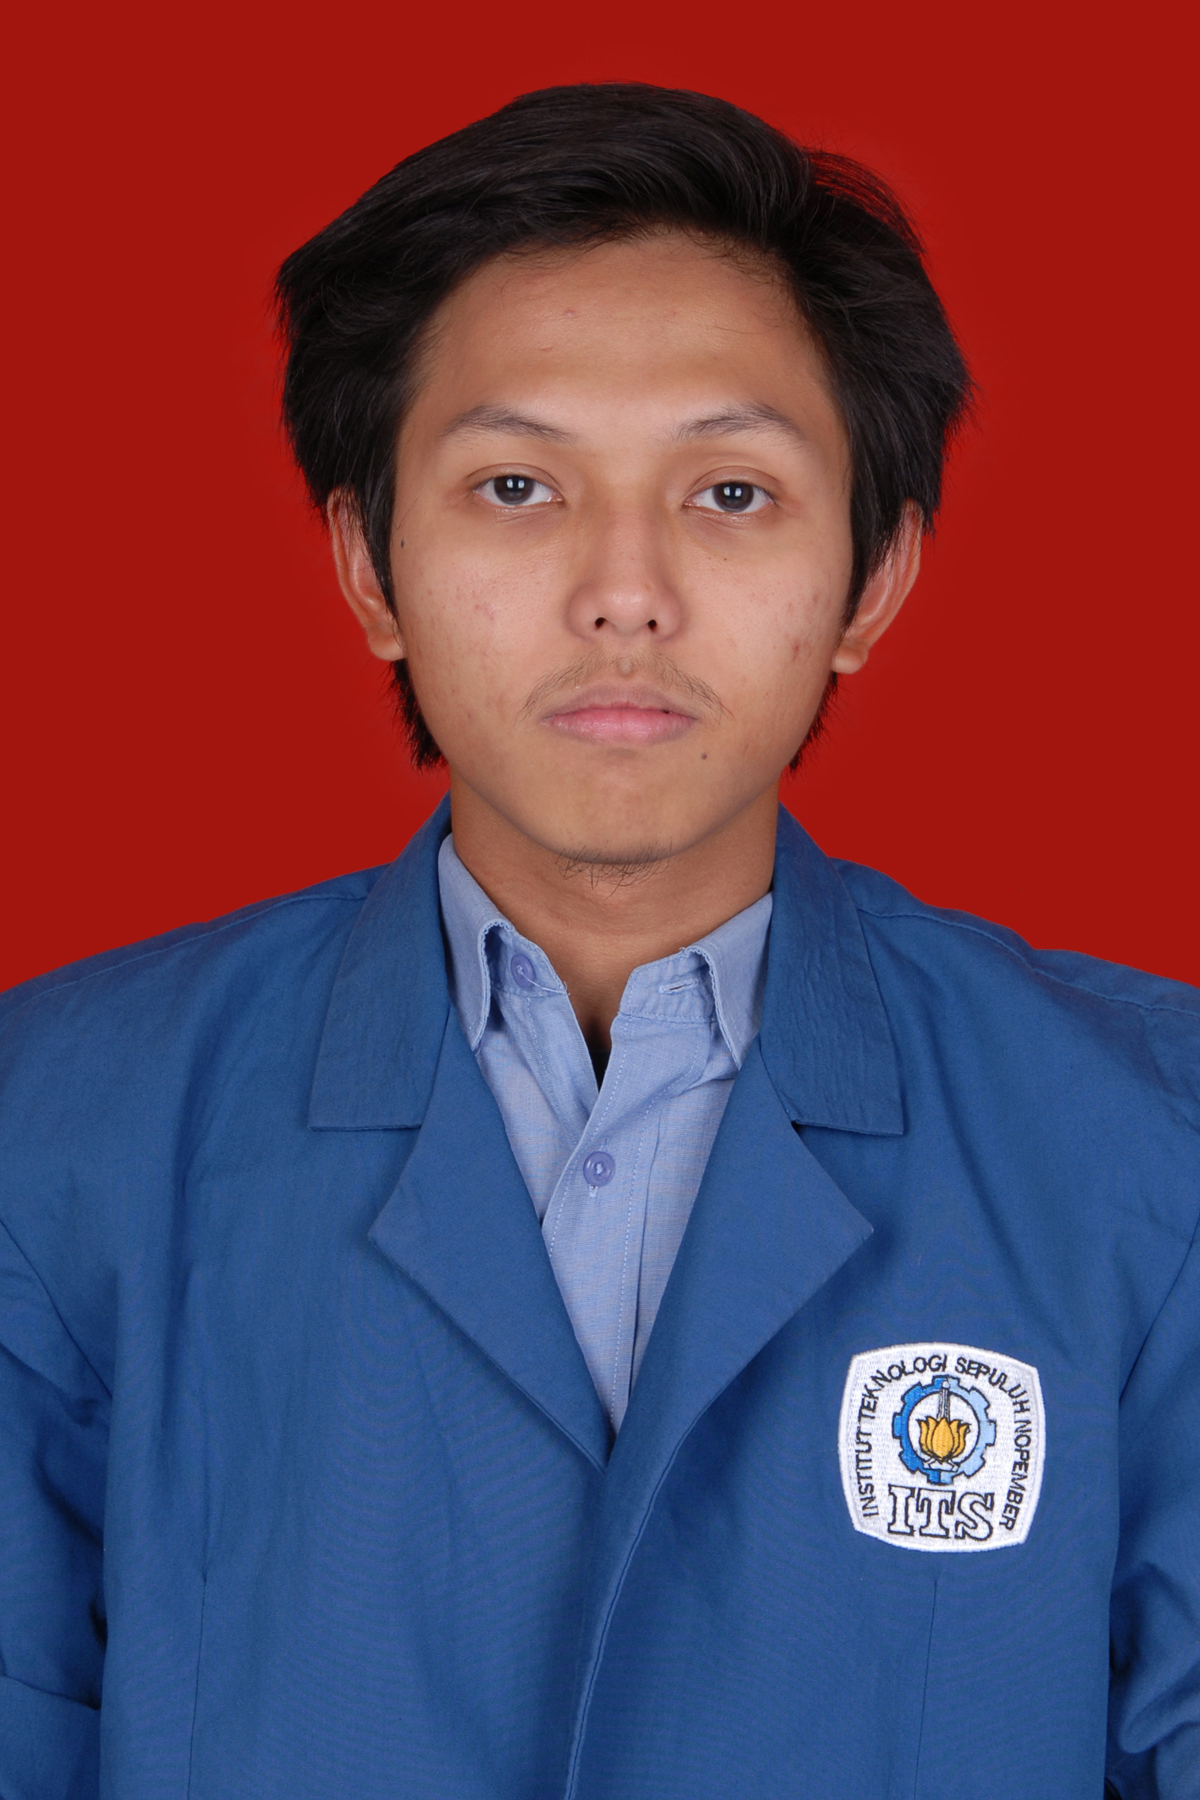
\includegraphics[width=0.29\textwidth]{images/cover/pic}
		\end{wrapfigure}
		\textbf{Fourir Akbar}, akrab dipanggil Oing, lahir pada tanggal 25 April 1996 di Surabaya. Penulis merupakan seorang mahasiswa yang sedang menempuh studi di Departemen Informatika Institut Teknologi Sepuluh Nopember. Memiliki beberapa hobi antara lain futsal dan DOTA. Pernah menjadi asisten dosen pada mata kuliah sistem operasi dan mata kuliah jaringan komputer pada semester 2016/2017 dan 2017/2018. Lalu juga pernah menjadi asisten dosen pada mata kuliah sistem terdistribusi pada tahun ajaran 2017/2018. Penulis juga pernah menjadi asisten dosen pendidikan informatika dan komputer terapan (PIKTI) ITS pada tahun ajaran 2016/2017 dan 2017/2018. Selama menempuh pendidikan di kampus, penulis juga aktif dalam organisasi kemahasiswaan, antara lain sebagai Staff Departemen Hubungan Luar Himpunan Mahasiswa Teknik Computer-Informatika pada tahun ajaran 2015/2016. Penulis juga aktif dalam kepanitiaan Schematics, antara lain sebagai Staff Biro Revolutionary Entertainment and Expo with Various Arts pada tahun ajaran 2015/2016 dan menjadi Badan Pengurus Harian (BPH) Biro Perlengkapan dan Transportasi pada tahun 2016/2017. Penulis juga merupakan salah satu administrator aktif pada Laboratorium Arsitektur dan jaringan Komputer di Departemen Informatika ITS.
\end{document}

\end{document} % YAY, WELCOME TO REAL WORD :)
